\section{Systemmodelle}

\subsection{Systemdiagramm}

\begin{figure}[H]
    \centering
    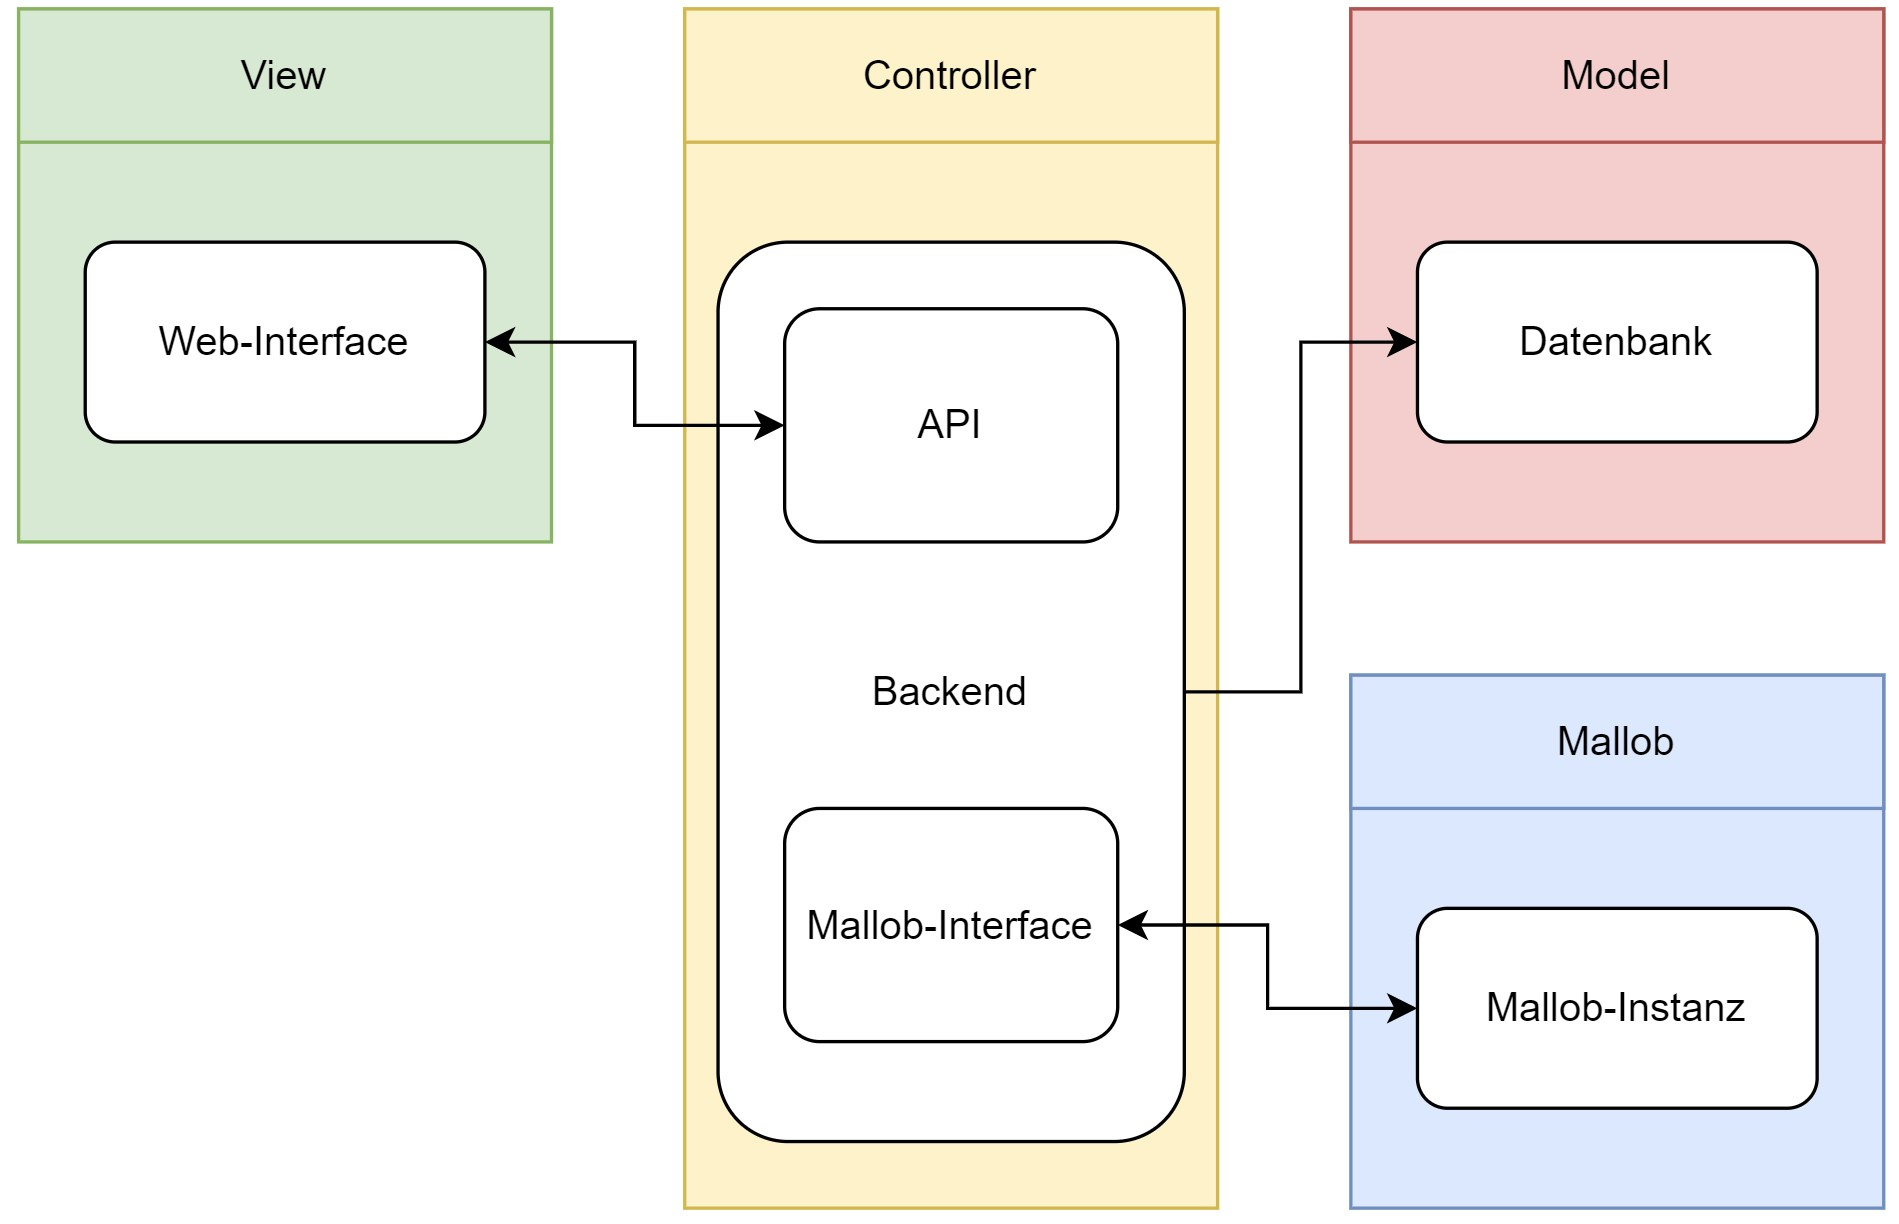
\includegraphics[width=\textwidth]{images-interface/Diagramme/Systemdiagramm3.jpg} \\
    \caption{\gls{Model-View-Controller}}
\end{figure}
Das System kann semantisch in 3 Komponenten gegliedert werden; View, Controller sowie Model. \\
Die Aufgabe des \textbf{Views}, bzw. des Web-Interfaces ist es dabei eine interaktive, grafische Benutzeroberfläche für die Interaktion mit Mallob bereitzustellen. \\
Der \textbf{Controller}, bzw. \gls{API} sowie Backend (Anfragen gehen über \gls{API} an das Backend) sind für die Kommunikation zwischen \gls{Datenbank}, Mallob und \gls{Web-Interface}, bzw. \gls{Nutzer} zuständig. Das Mallob-Interface ist im Backend implementiert und für die Kommunikation zwischen der Backend-Logik und einer laufenden Mallob-Instanz zuständig.\\
Im \textbf{Model} hält eine \gls{Datenbank} die \hyperref[PD]{Daten des Systems}. \\
\textbf{Extern} liegt die laufende Mallob-Instanz. Mallob ist nicht Teil unseres Systems. Unser System kommuniziert lediglich mit Mallob.

\pagebreak

\subsection{Anwendungsfalldiagramme}

\begin{figure}[H]
    \centering    
    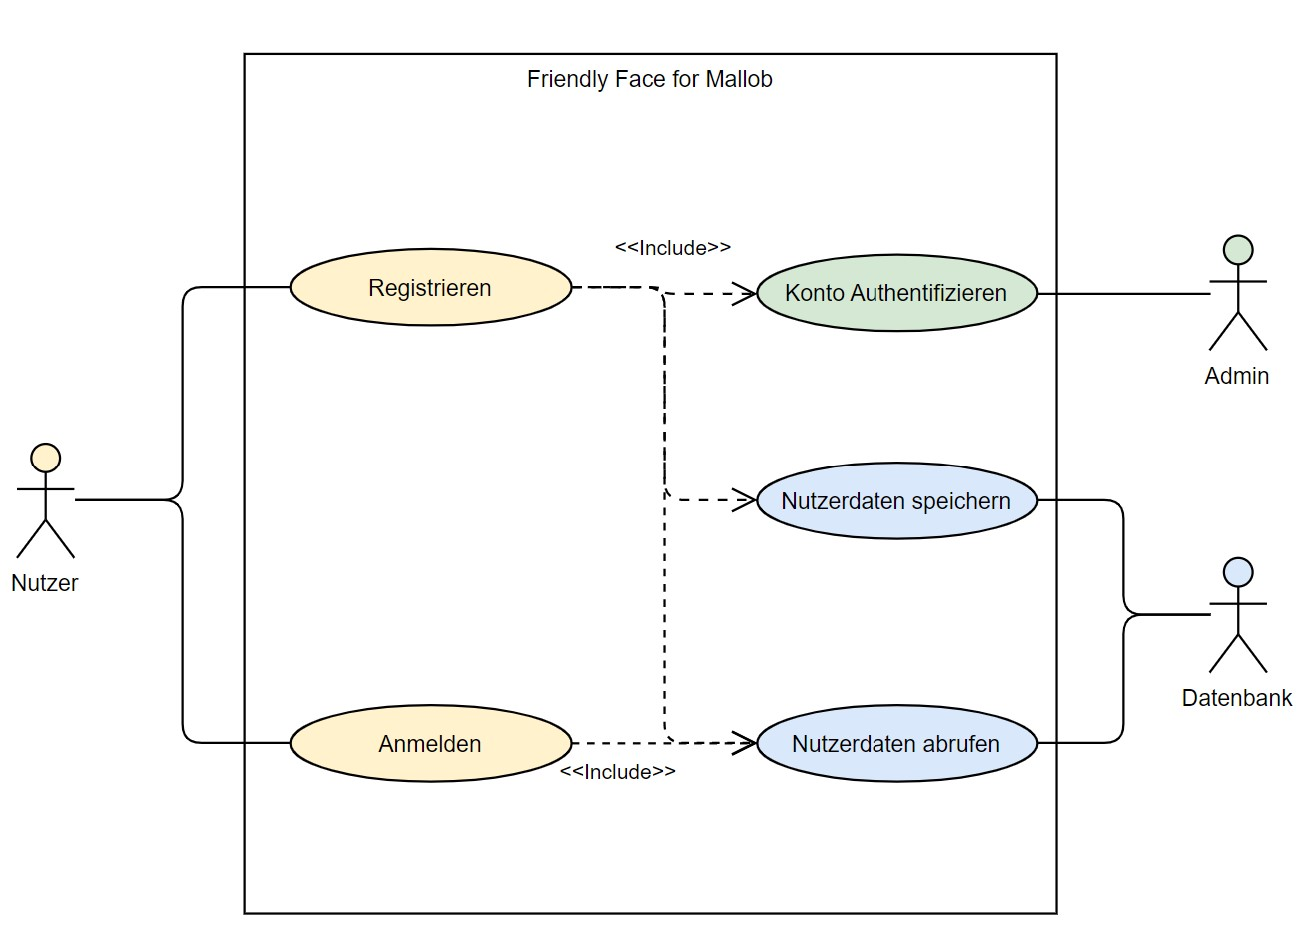
\includegraphics[width=\textwidth]{images-interface/Diagramme/Login_register_3_screenshot.jpg} 
    \caption{Registrierung von \gls{Nutzer}n}
\end{figure}


Registriert sich ein \gls{Nutzer} gemäß \hyperref[FA:API:Registrierung von Nutzern]{F1150}, so wird seine Registrierunganfrage von einem \gls{Administrator} verifiziert. Die \gls{Datenbank} speichert die \hyperref[PD:Nutzerdaten]{Nutzerdaten}.\\
Möchte sich ein registrierter \gls{Nutzer} im \gls{Web-Interface} anmelden, so werden die Nutzerdaten aus der \gls{Datenbank} geholt und mit den eingegebenen Daten verglichen.



\begin{figure}[H]
    \centering
    \includegraphics[width=\textwidth]{images-interface/Diagramme/Request_authntification_screenshot.jpg}
    \caption{Authentifizierung von \gls{API}-Anfragen}
\end{figure}
Jede Anfrage an die \gls{API} muss authentifiziert werden. Dies geschieht, indem der \gls{Authentifizierungstoken}, der mit der Anfrage geschickt wurde, mit dem in der \gls{Datenbank} gespeichertem \gls{Authentifizierungstoken} abgeglichen wird. Wurde eine Anfrage authentifiziert, also sichergestellt, das der \gls{Nutzer} diese auch ausführen darf, so wird sie weiterverarbeitet.\\
Jede Anfrage an die \gls{API} wird für eine gewisse Zeit gespeichert, um sie später noch einmal referenzieren oder einsehen zu können.

\pagebreak

%https://www.overleaf.com/project
\begin{figure}[H]
    \centering
    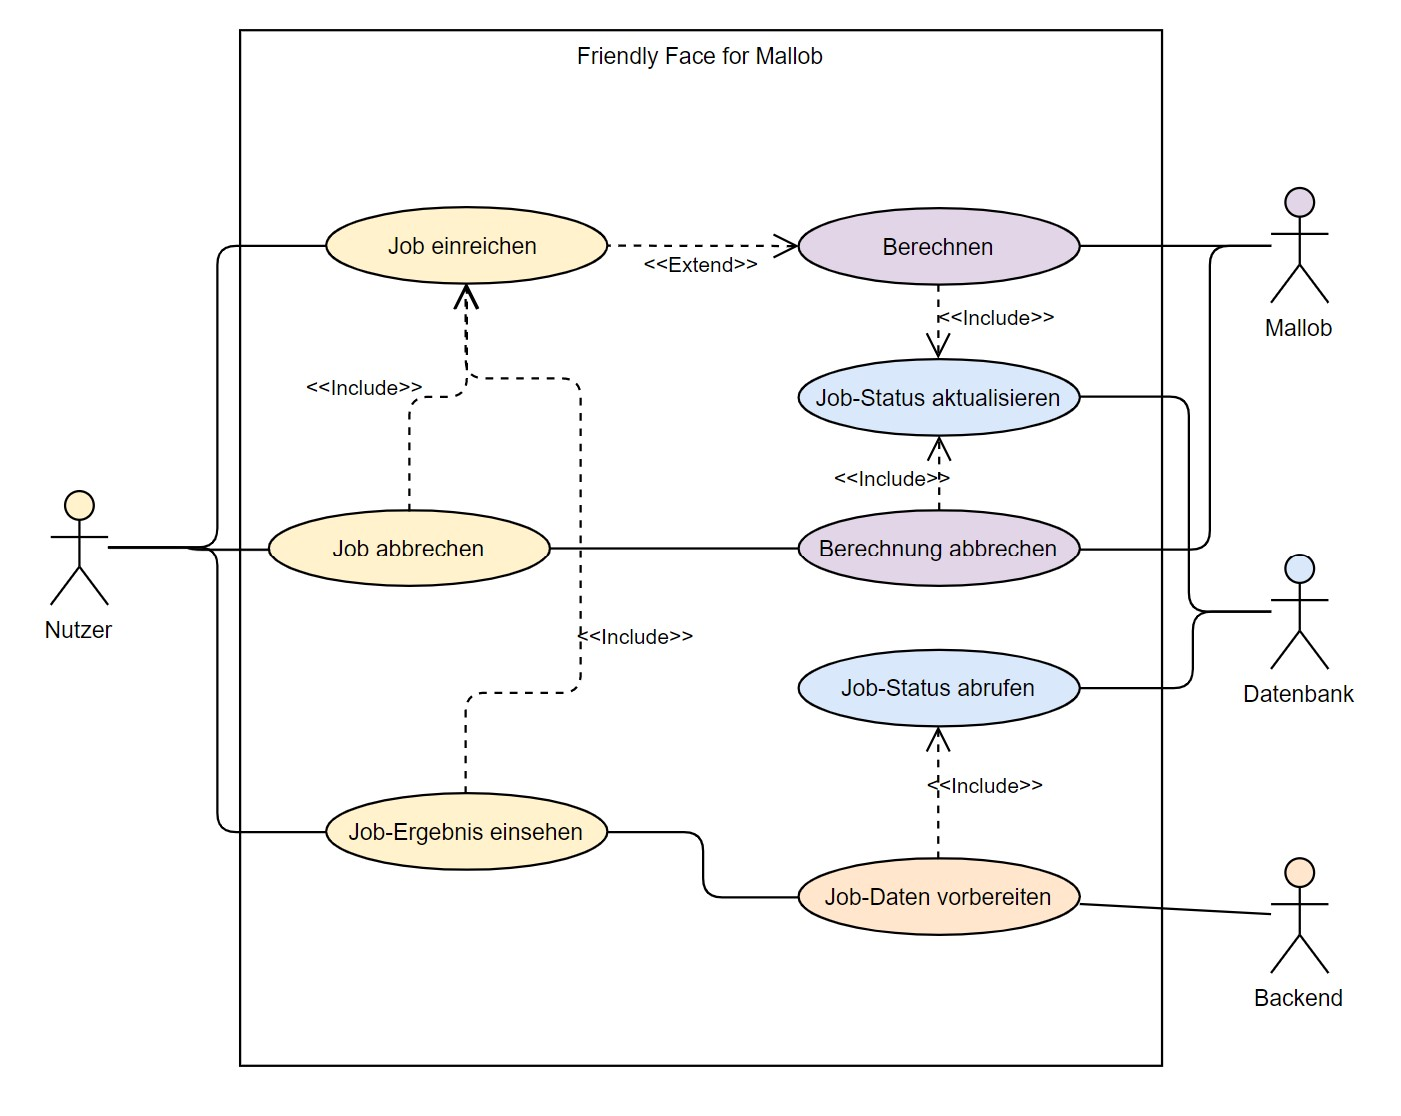
\includegraphics[width=\textwidth]{images-interface/Diagramme/Submit-abort-view-screenshot.jpg}
    \caption{Einreichen, Abbrechen und Einsehen von \hyperref[B:Jobs]{Jobs}}
\end{figure}

Reicht ein \gls{Nutzer} ein \hyperref[B:Jobs]{Job} ein, so wird dieser (je nach Konfiguration) von Mallob bearbeitet. Mallob gibt dabei Rückmeldung über den Job-Status, also entweder das Ergebnis des \hyperref[B:Jobs]{Jobs}, oder ob ein Fehler aufgetreten ist. Dieser Status wird in der \gls{Datenbank} gespeichert. \\
Ein \gls{Nutzer} kann die Bearbeitung eines \hyperref[B:Jobs]{Jobs}, der gerade von Mallob berechnet wird, abbrechen. Die berechneten Zwischenergebnisse werden dann gespeichert und können später abgerufen werden. \\
Möchte ein \gls{Nutzer} einen \hyperref[B:Jobs]{Job} einsehen, so ist es wichtig das dieser bereits eingereicht wurde. Um ein \hyperref[B:Jobs]{Job} einsehen zu können werden zunächst die angeforderten \hyperref[B:Job-Informationen]{Job-Informationen} aus der \gls{Datenbank} geholt und dann vorbereitet an den \gls{Nutzer} geschickt.


%\begin{center}
%    \includegraphics[scale=0.6]{images-interface/Request_authntification_screenshot.jpg} \\
%    Anwendungsfalldiagramm 2: Authentifizierung von \gls{API}-Requests
%\end{center}


\begin{figure}[H]
    \centering
    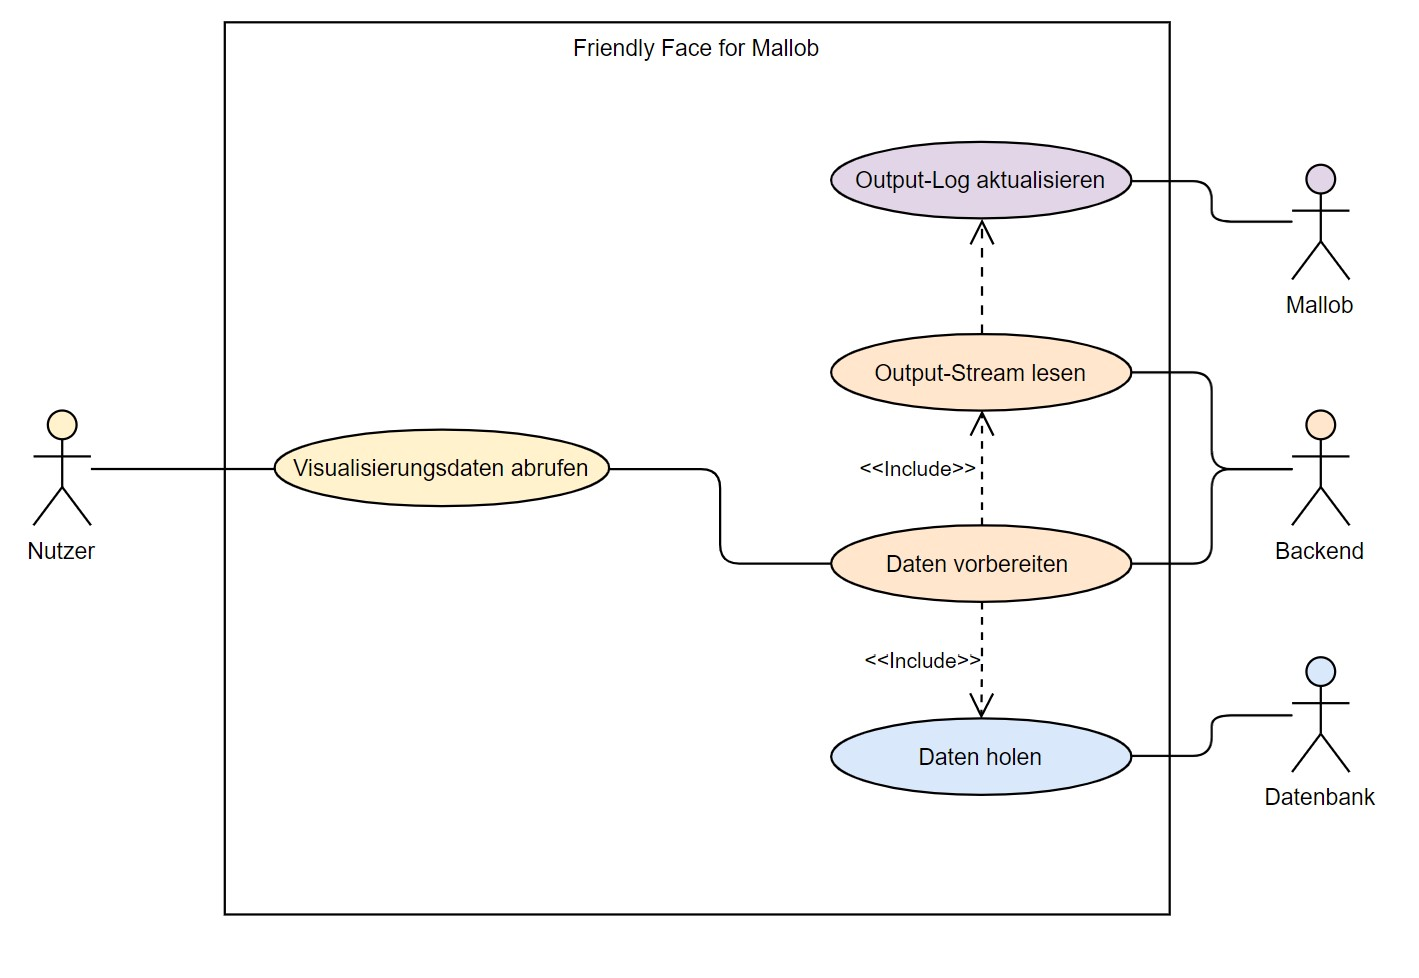
\includegraphics[width=\textwidth]{images-interface/Diagramme/visualisierungsdaten_anwendungsfaelle.jpg}
    \caption{Mallob-Visualisierungsdaten abrufen}
\end{figure}
Möchte ein \gls{Nutzer} Mallob-Visualisierungsdaten abrufen, so holt das System bereits vergangene Events aus der \gls{Datenbank}, um daraus die Daten für die Visualisierung vorzubereiten. Des weiteren wird live der Output-\gls{Stream} der \gls{Log-Datei} von Mallob ausgelesen, um Echtzeit-Visualisierung für den \gls{Nutzer} anzubieten. 


\pagebreak

\subsection{Aktivitätsdiagramme}
\begin{figure}[H]
    \centering
    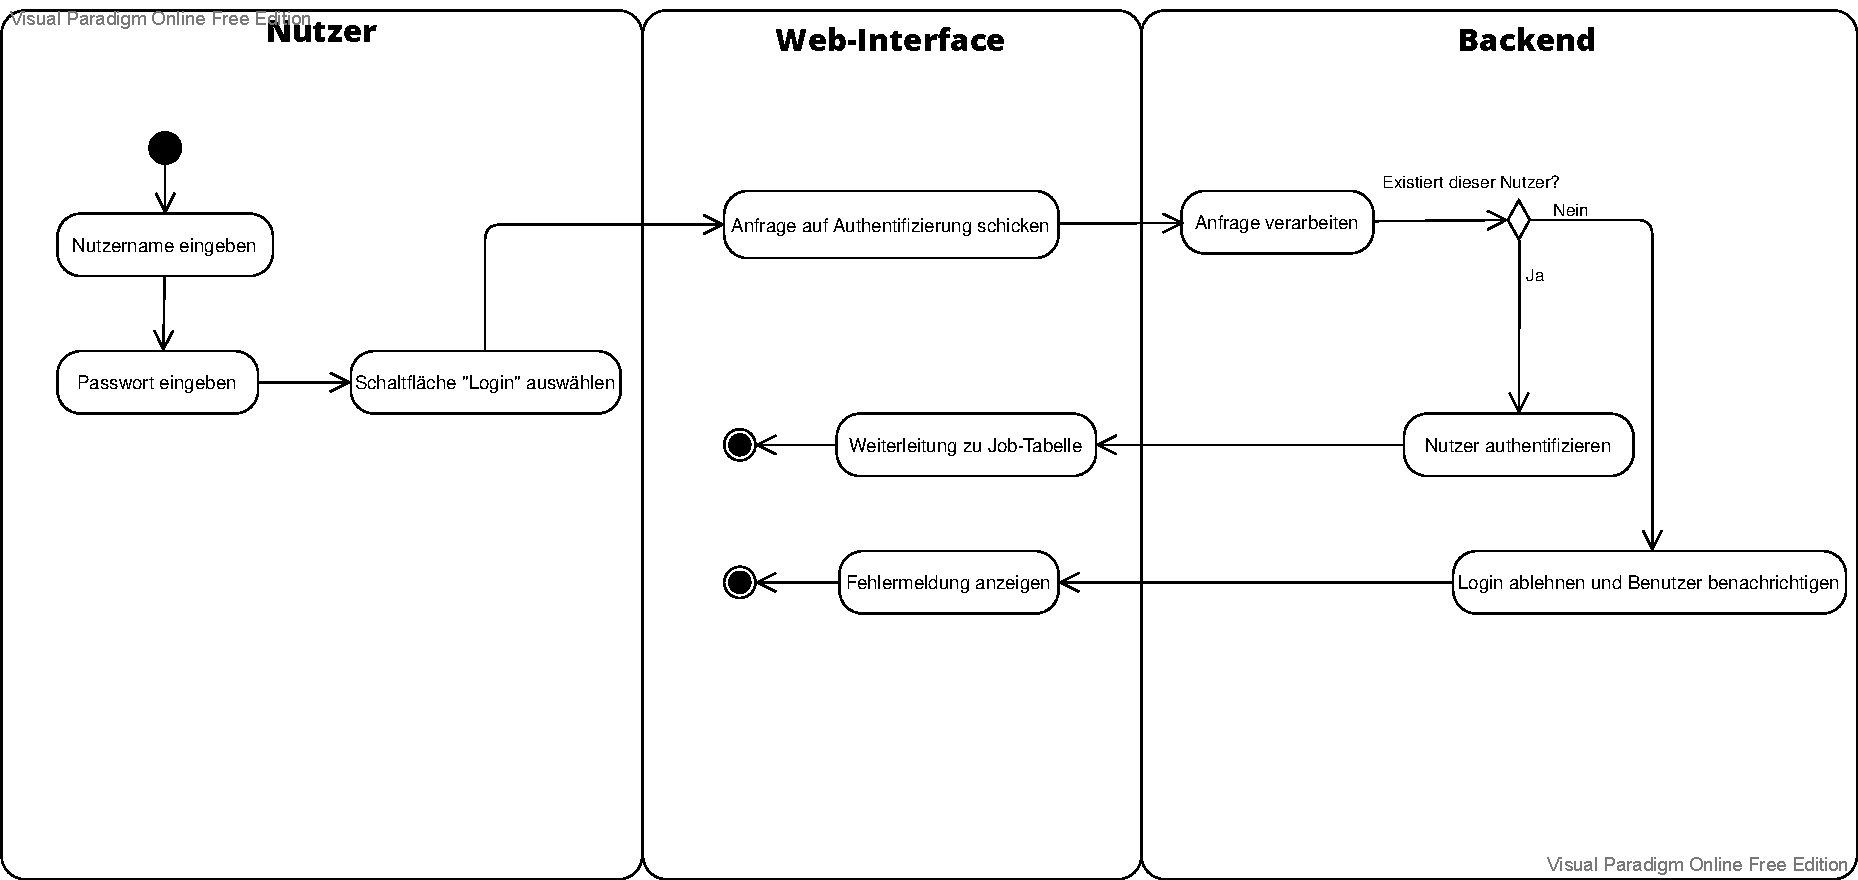
\includegraphics[width=\textwidth]{images-interface/v3_aktivitaetsdiagramme/Anmelden_v10.pdf}
    \caption{Anmeldung im System über das \gls{Web-Interface}}
    \label{fig:login_activity}
    
\end{figure}
Ein \gls{Nutzer} muss sich anmelden, um die Funktionen des \gls{Web-Interface}s zu benutzen. Zuerst gibt der \gls{Nutzer} über die Eingabe-Maske seinen Nutzernamen und Passwort ein und klickt auf die Schaltfläche \enquote{login}, wobei das \gls{Web-Interface} seine Anfrage zur Authentifizierung an die \gls{API} schickt. Die \gls{API} überprüft die Daten und hat zwei Möglichkeiten: Entweder existiert der \gls{Nutzer} mit diesen Anmelde-Daten im System, er wird authentifiziert und das \gls{Web-Interface} leitet ihn zur Job-Tabelle weiter, oder die Anmelde-Anfrage wird abgelehnt und das \gls{Web-Interface} zeigt dem \gls{Nutzer} eine Fehlermeldung.


\begin{figure}[H]
    \centering
    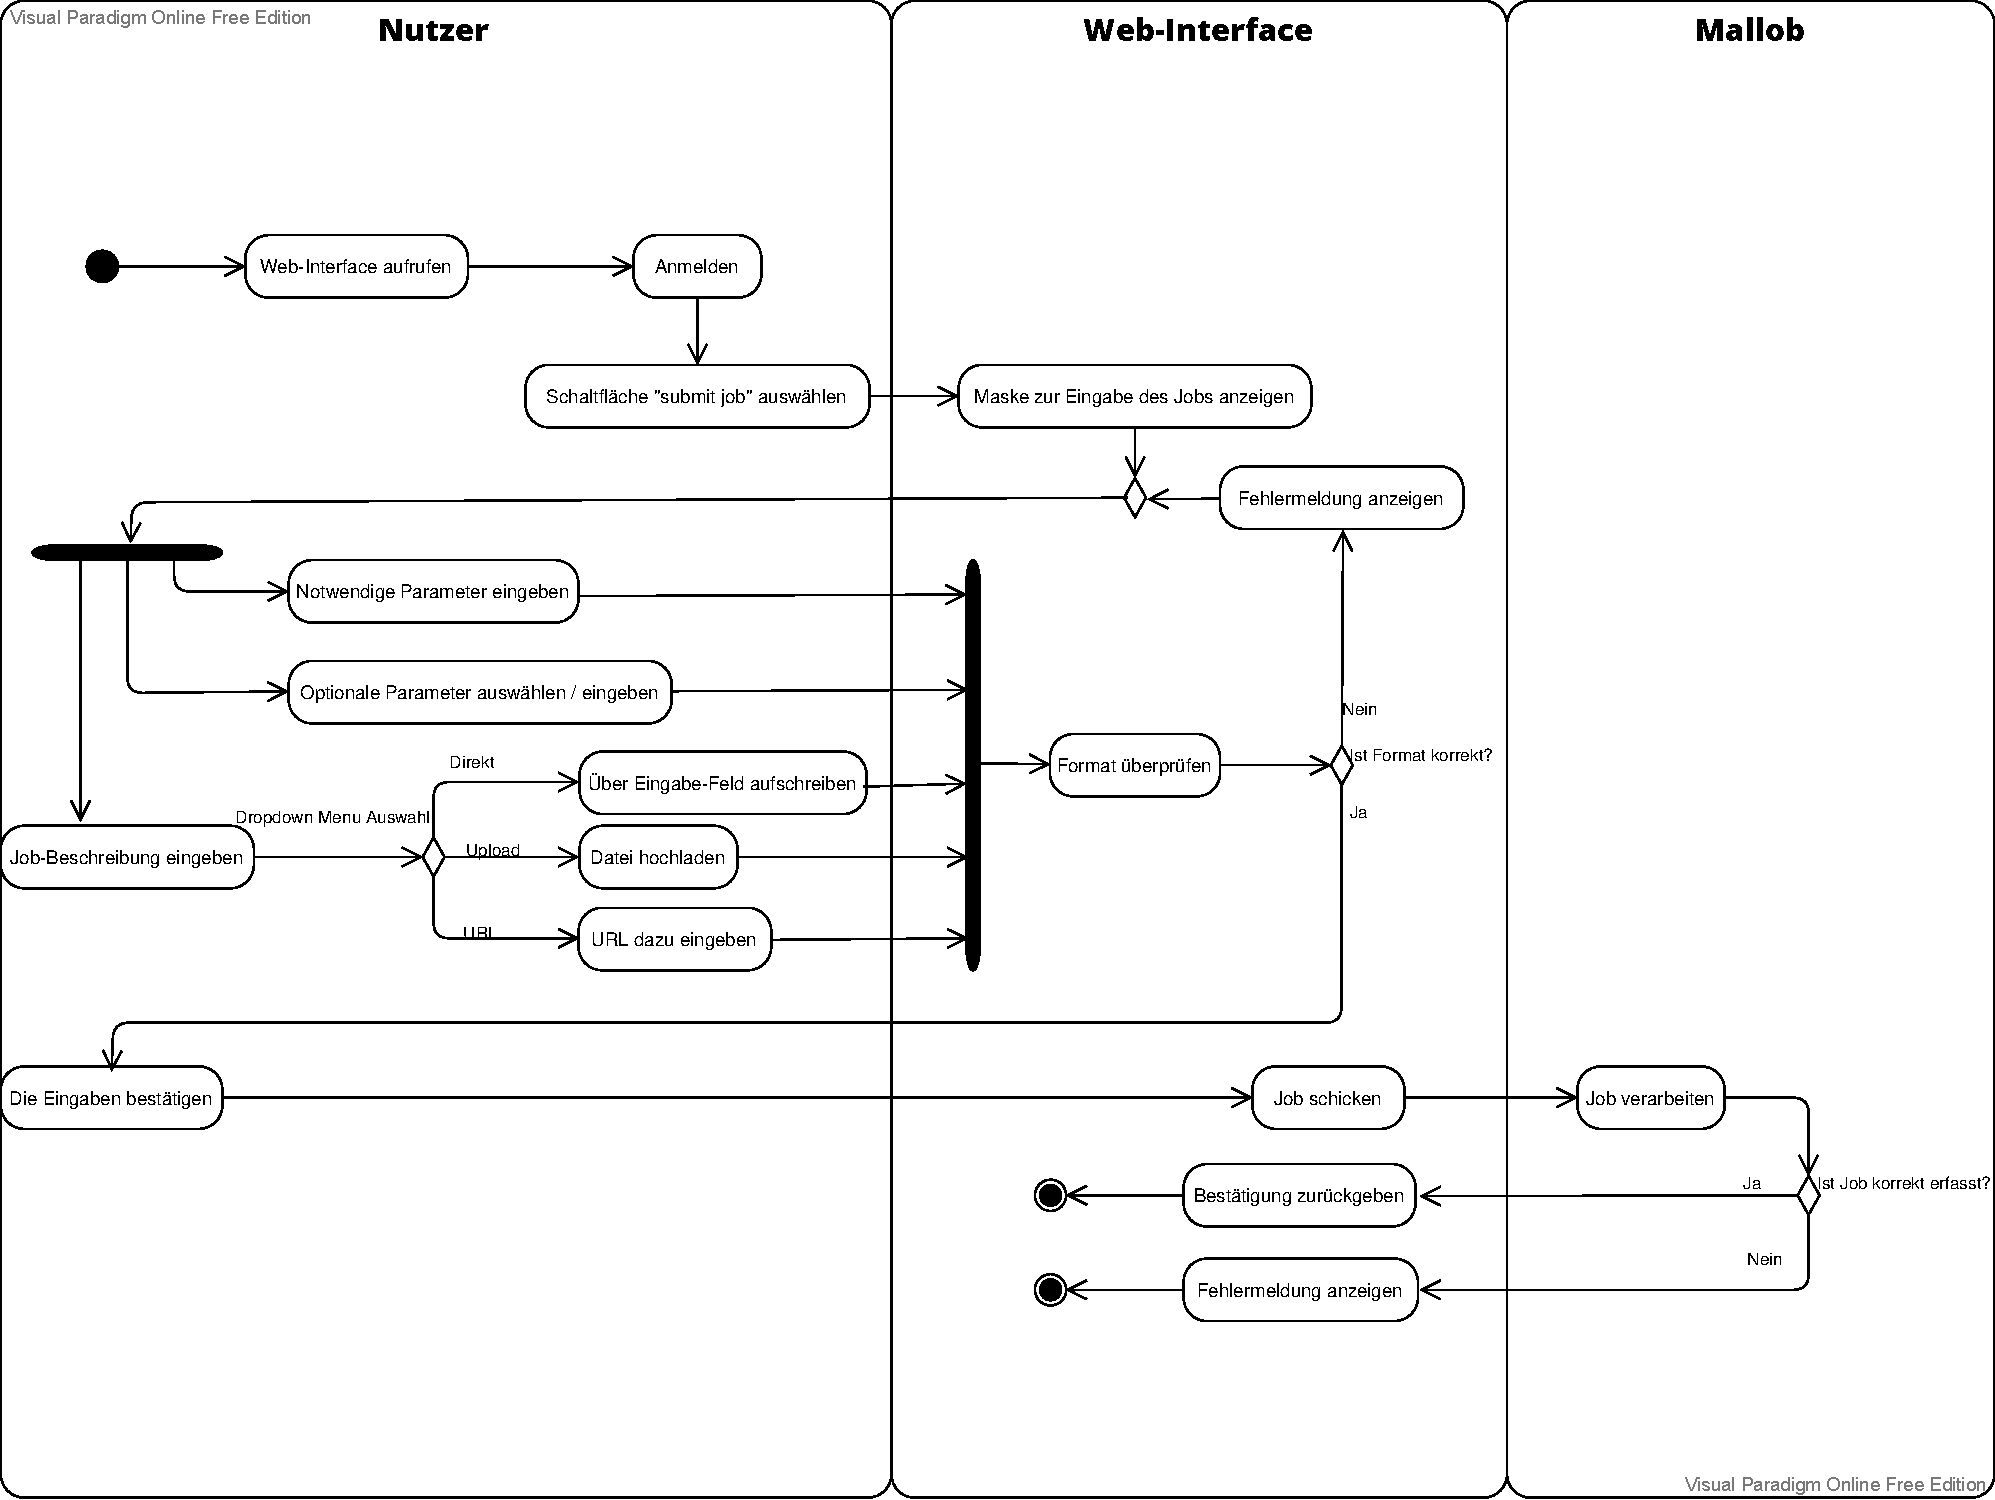
\includegraphics[width=\textwidth]{images-interface/v3_aktivitaetsdiagramme/Job_einreichen_v11.pdf}
    \caption{Einreichen eines \hyperref[B:Jobs]{Jobs} über das \gls{Web-Interface}}
\end{figure}
Möchte ein \gls{Nutzer} \hyperref[B:Jobs]{Jobs} einreichen, muss er angemeldet sein. Zunächst wählt er die Schaltfläche \enquote{submit job}. Daraufhin zeigt das \gls{Web-Interface} eine \hyperref[pages:submit-job]{Eingabe-Maske} angezeigt. Hier muss er die notwendigen Optionen eingeben, die gewünschten optionalen Optionen auswählen und die \hyperref[B:Job-Beschreibung]{Job-Beschreibung} auf genau eine der drei Weisen übergeben. Über ein \gls{Dropdown-Menue}, wählt er zwischen direkter Eingabe, hochladen einer Datei, die die Beschreibung enthält oder Angabe einer URL. Nach Bestätigung der Eingabe wird das Format der Eingaben vom \gls{Web-Interface} überprüft. Falls das Format inkorrekt war, muss der \gls{Nutzer} die inkorrekte Eingabe verändern, andernfalls kann der \gls{Nutzer} die Eingaben bestätigen, was seine \hyperref[B:Jobs]{Job} über das \gls{Web-Interface} zu Mallob schickt. Mallob überprüft die \hyperref[B:Job-Beschreibung]{Job-Beschreibung} und die \hyperref[B:Job-Konfiguration]{Job-Konfiguration}. Falls diese fehlerhaft sind, wird eine Fehlermeldung vom \gls{Web-Interface} angezeigt. Falls die Daten des \hyperref[B:Jobs]{Jobs} vom \gls{Nutzer} im korrekten Format eingegeben wurden, wird eine Bestätigung zur \hyperref[B:Jobs]{Job}-Bearbeitung vom \gls{Web-Interface} zurückgegeben.

\begin{figure}[H]
    \centering
    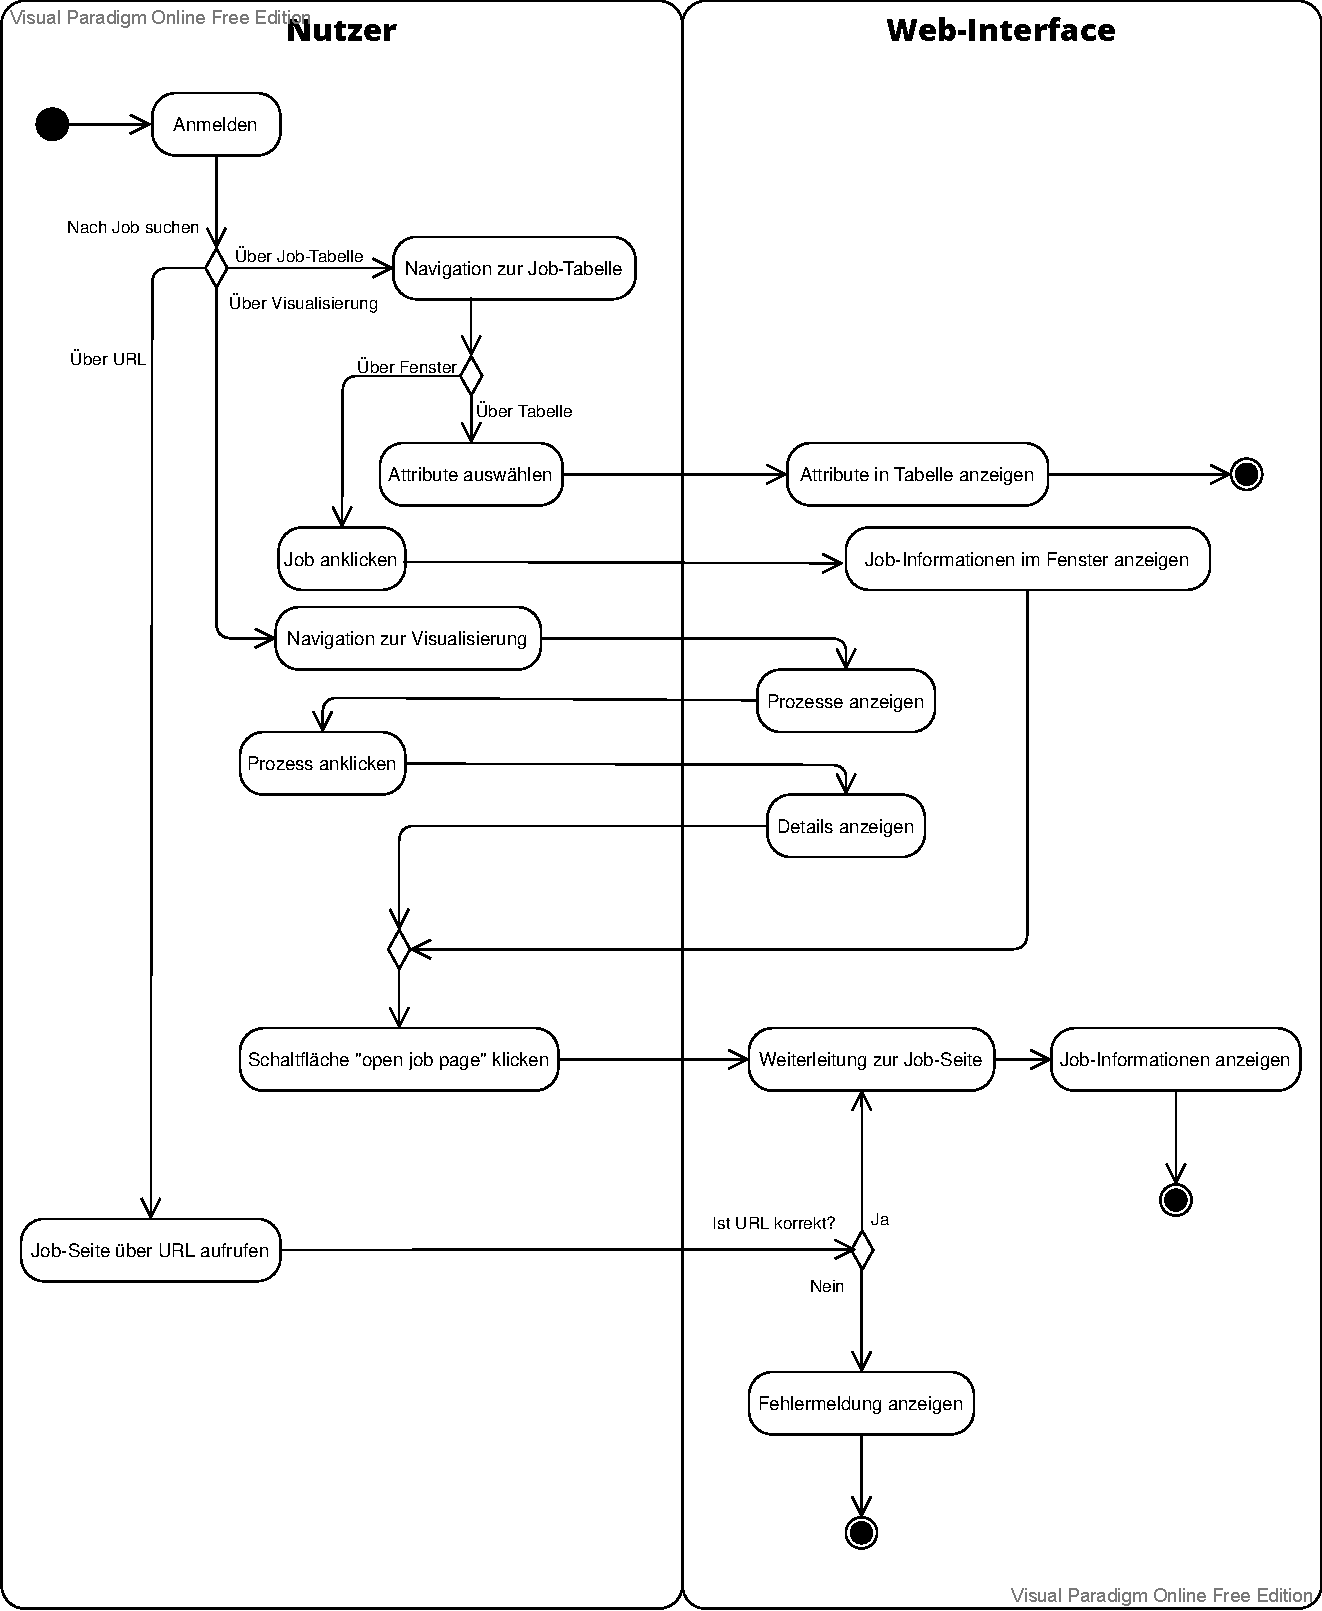
\includegraphics[width=\textwidth]{images-interface/v3_aktivitaetsdiagramme/Get_information_v3.pdf}
    \caption{Einsehen von \hyperref[B:Job-Informationen]{Job-Informationen}}
\end{figure}
\newpage
Hier werden die verschiedene Wege zum Einsehen der \hyperref[B:Job-Informationen]{Job-Informationen} angezeigt. Zuerst muss immer ein \gls{Nutzer} dafür angemeldet sein. Dann hat er 3 Möglichkeiten: 
\begin{enumerate}
   

\item Der \gls{Nutzer} gibt die URL einer Job-Seite im Browser ein und wird auf diese weitergeleitet, wo ihm die \hyperref[B:Job-Informationen]{Job-Informationen} angezeigt werden.

%[TODO]  : was ist der satz bei 2.? Was ist PE
\item Der \gls{Nutzer} klickt die Schaltfläche \enquote{Visualization} an. Danach klickt er auf einen Prozess und es werden die Details dazu angezeigt. Dann klickt er auf die Schaltfläche \enquote{open job page}, was ihn zur Job-Seite weiterleitet und ihm da die \hyperref[B:Job-Informationen]{Job-Informationen} anzeigt werden.

\item Der \gls{Nutzer} navigiert zur Job-Tabelle, die seine eingereichten \hyperref[B:Jobs]{Jobs} enthält. Hier kann er entweder ein Attribut aus dem \gls{Dropdown-Menue} auswählen, welches dann in der Tabelle als Spalte angezeigt wird, oder er klickt einen der angezeigten \hyperref[B:Jobs]{Jobs} an und die \hyperref[B:Job-Informationen]{Job-Informationen} werden in einem nebenstehenden Fenster angezeigt. Hier kann man ebenfalls die Schaltfläche \enquote{open job page} wählen, was ihn zu Job-Seite weiterleitet und da die \hyperref[B:Job-Informationen]{Job-Informationen} anzeigt.
\end{enumerate}